\documentclass[10pt]{examdesign}
\usepackage{amsmath}
\usepackage{enumitem}
\usepackage{amsfonts}
\usepackage{pgfplots}
\usepackage{pifont}
\usepackage{graphicx}
\usepackage{fancyhdr}
\usepackage{cancel}
\usepackage{gensymb}
\usepackage[american]{circuitikz}

\SectionFont{\large\sffamily}
\Fullpages
\ContinuousNumbering
\usepackage{ulem}
\ProportionalBlanks{2}


\DefineAnswerWrapper{}{}
\NumberOfVersions{1}
%\IncludeFromFile{foobar.tex}
\examname{\Large{Semester 1 Exam}}
\class {\Large Physics}

\def \namedata {Name: \hrulefill\\ 
	Date: \hrulefill \\
	Period: \hrulefill \\

			\begin{tabular}{| p{1cm} | p{1cm} | p{1 cm} | p{1cm} |}
	\hline
		+1 & 0 & -1 & $\Sigma$ 
		\\
		\hline
		& & & \vspace{.5cm}
		\\ \hline
	
	\end{tabular}
	\\
 \vspace{-.6in}
	
}




\begin{document}




\begin{multiplechoice} [title={Multiple Choice},
	rearrange=no]


	
	\begin{question}
A blue sphere and a red sphere with the same diameter are released from rest at the top of a ramp. The red sphere takes a longer time to reach the bottom of the ramp. The spheres are then rolled off a horizontal table at the same time with the same speed and fall freely to the floor. Which sphere reaches the floor first?
\choice{The red sphere}
\choice{The blue sphere}
\choice{The sphere with the greater mass}
\choice{Neiher; the spheres reach the floor at the same time.}
	\end{question}



\begin{question}
	An elevator carrying a person of mass m is moving upward and speeding up. How does the magnitude $F$ of the force exerted on the person by the elevator floor compare with the magnitude $mg$ of the gravitational force?
	\choice{$F = mg$}
	\choice{$F > mg$}
	\choice{$F < mg$}
	\choice{It depends on the speed of the elevator.}
\end{question}



\begin{question}
	An athlete sitting in a wheelchair at rest throws a basketball forward. Since the athlete and the wheelchair have greater mass than the basketball has, the athlete and the wheelchair will — 
\choice{move backward at a lower speed than the basketball moves forward}
\choice{travel the same distance as the basketball but in the opposite direction}
\choice{move backward at a higher speed than the basketball moves forward}
\choice{move forward faster than the basketball moves forward.}
\end{question}


\begin{question}
	The Voyager 2 Spacecraft was launched on August 20 1977.  It flew past the planets Jupiter, Saturn, Uranus and Neptune.  Though it has no fuel left, it continues to fly away from the earth, and is currently twice as far from the sun as the dwarf planet Pluto.  If it is left alone, it will pass close to the star Sirius in the year 298,000.  Which statement best explains why Voyager 2 continues to travel farther from the earth?
	\choice{For every action, there is an equal, opposite reaction.}
	\choice{The force of the solar wind on its solar panels is blowing Voyager 2 through space at a constant speed.}
	\choice{Objects in motion will remain in motion unless acted upon by an external, unbalanced force.}
	\choice{A Force on an object is equal to the mass of the object times its acceleration.}
\end{question}

\begin{question}
	Billy-Bob is showering in the locker room after a football game when he drops the soap.  The soap slides all the way across the locker room without a significant decrease in speed, and does not stop until it hits the wall.  This is because - 
\choice{The soap is converting internal thermal energy into work.}
\choice{There is very little friction between wet soap and a smooth floor.}
\choice{The air in the room pushes the soap across the floor.}
\choice{The ground puts an impulse on the soap, causing the soap to increase its momentum.  }
\end{question}

\begin{question}
	Homer is 15 meters from Barney, who has just stolen Homer's keys.  Homer is running at a speed of 5 m/s and Barney is running at a speed of 3 m/s.  How long will it take Homer to catch up to Barney?
	\choice{1.875 s}
	\choice{7.5 s }
	\choice{15 s}
	\choice{He will never catch up.}
\end{question}


\begin{question}
A book is at rest on top of a table. Which of the following is correct?
\choice{The book is in equilibrium.}
\choice{The book has no inertia.}
\choice{The inertia of the book is equal to the inertia of the table.}
\choice{There is no force acting on the table. }
\end{question}

\begin{question}
	An astronaut is standing on the moon.  He holds a hammer in one hand and a feather in the other.  What happens when he lets them go, and why?
	\choice{The hammer lands first because it is heavier.}
	\choice{The feather lands first because there is no air resistance on it.}
	\choice{Both objects land at the same time because they both experience the same acceleration due to gravity.}
	\choice{Both objects float away because there is no gravity on the moon.}
\end{question}


\begin{question}
	An airplane is traveling at a constant horizontal speed, and is ascending at a rate of 2 m/s. How do the forces of Lift and Weight compare?	
\choice{Lift > Weight}
\choice{Lift = Weight}
\choice{Lift < Weight}
\choice{It cannot be determined.}
\end{question}

\begin{question}A stream is flowing to the north at 0.3 m/s.  A duck swims in the stream, and paddles directly to the east at 0.4 m/s. What is the resultant speed of the duck relative to a person standing on shore?  
\choice{0.2 m/s}
\choice{0.3 m/s}
\choice{0.4 m/s}
\choice{0.5 m/s}
\end{question}

\begin{question}
	Two tug of war teams pull on opposite ends of a rope:
	
	\begin{center}
			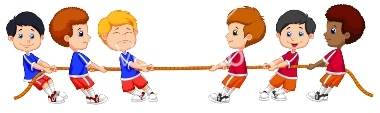
\includegraphics[height={.5in}]{tug.png}
	\end{center}

	
	 Each team exerts a horizontal force of 5000 N.  If the mass of the entire system is 500 kg, the acceleration of the system will be - 
	\choice{0 m/s\textsuperscript{2}}
	\choice{0.1 m/s\textsuperscript{2}}
	\choice{10 m/s\textsuperscript{2}}
	\choice{20 m/s\textsuperscript{2}}
\end{question}




\begin{question}
A bowling ball at a height of 36 meters above the ground is falling vertically at a rate of 12 meters per second. Which of these best describes what will happen to it? *
\choice{It will hit the ground in exactly three seconds at a speed of 12 m/s.}
\choice{It will hit the ground in less than three seconds at a speed greater than 12 m/s.}
\choice{It will hit the ground in more than three seconds at a speed less than 12 m/s.}
\choice{It will hit the ground in less than three seconds at a speed less than 12 m/s.}
\choice{It will hit the ground in more than three seconds at a speed greater than 12 m/s.}
\end{question}

\begin{question}
	In a movie, a criminal is trying to escape from the police by driving at 55 m/s. The police are driving at a speed of 60 m/s.  If the criminal is 500 m from the police, how long will it take the police to catch up to the criminal?  
	\choice{1.818 s}
	\choice{8.333 s}
	\choice{12 s}
	\choice{100 s}
	\choice{The police will never catch up.}
\end{question}



\begin{question}
	A marble rolls off the top of a flat, level roof with an initial velocity of 2.5 m/s.  If the height of the building is 10 meters, what is the horizontal component of the marble's velocity when it hits the ground?
\choice{2.5 m/s}
\choice{12 m/s}
\choice{14.007 m/s}
\choice{16.5 m/s}
\choice{It cannot be determined without knowing the mass of the marble.}
\end{question}




\begin{question}
	A ball rolls off a cliff with an initial velocity of 12 m/s.  It lands 14.5 meters away.  How tall was the cliff?
	\choice{1.2 m}
	\choice{7.161 m}
	\choice{14.5 m}
	\choice{117.6 m}
	\choice{There is not enough information}
\end{question}

\begin{question}
Sara throws the same ball four times.  The trajectories are shown below. Assuming that air resistance is negligible, which ball stayed in the air the longest? 

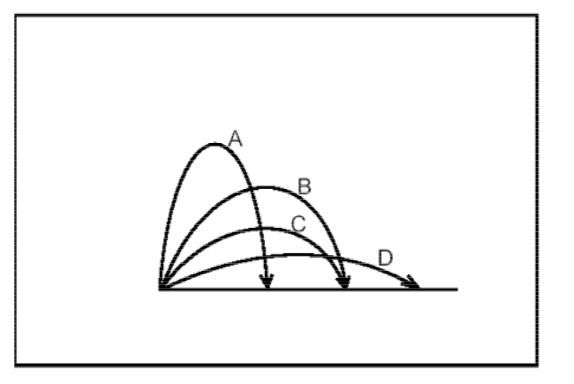
\includegraphics[height={1in}]{proj.png}

\choice{A}
\choice{B}
\choice{C}
\choice{D}
\choice{All were in the air for the same amount of time.}
\end{question}






\begin{question}
	Two bicycle riders, Lance and Floyd, are racing each other. Lance has a greater top speed of 25 m/s, compared to Floyd's 20 m/s.  However, Floyd has a greater acceleration of 3 m/s\textsuperscript{2}, compared to Lance's 2 m/s\textsuperscript{2}.  Which of the riders will win the race?
\choice{Lance}
\choice{Floyd}
\choice{Either Lance or Floyd can win the race, depending on who has the more expensive bicycle.}
\choice{It is impossible to tell without knowing the masses of the riders.}
\choice{It is impossible to tell without knowing the distance they are riding.}
\end{question}




\begin{question}
Billy-Bob drops a watermelon out of a 2nd story window. It hits the ground at a speed of v. What would the speed of the watermelon be if he dropped it out of the 8th story window?
Mark only one oval.
\choice{v}
\choice{2v}
\choice{4v}
\choice{6v}
\choice{8v}
\end{question}

\begin{question}
	A train is traveling to the right with a constant speed $v_t$.  Two identical spheres are rolling on the floor of one train car.  In the frame of reference of the train, the spheres are moving directly toward each other with a speed $v_p$, parallel to the train's motion, as shown in the figure above.  A person is standing outside the train as it passes by.  What are the velocities that the person would measure of each of the spheres as the train passes by? 
	
	\begin{center}
		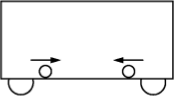
\includegraphics[height=0.5in]{train2.png}  
	\end{center}
	
	
	
	\choice{Left Sphere: $v_p + v_t$ \hspace{0.25in} Right sphere: $v_p + v_t$}
	\choice{Left Sphere: $v_p - v_t$ \hspace{0.25in} Right sphere: $v_p + v_t$}
	\choice{Left Sphere: $v_p + v_t$ \hspace{0.25in} Right sphere: $v_p - v_t$}
	\choice{Left Sphere: $v_p - v_t$ \hspace{0.25in} Right sphere: $v_p - v_t$}
	
\end{question}

\begin{question}
	A student standing on the roof of a 50-meter tall buliding kicks a stone with an initial horizontal speed of 4 m/s, as shown in the diagram.  How much time is required for the stone to reach the ground below? 
	\choice{3.19 s}
	\choice{5.10 s}
	\choice{10.2 s}
	\choice{12.5 s}
	
	\vspace{-1in} \hspace{2 in} 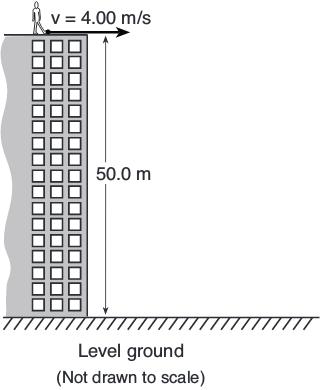
\includegraphics[height=1.1in]{building.png}
	
\end{question}


\begin{block}
	\textit{	The following two questions refer to the following information:}
	
	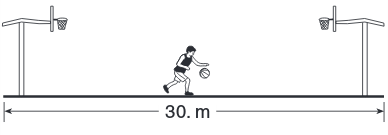
\includegraphics[height=0.5in]{bball.png} 
	
	During a drill in basketball practice, a player runs the length of a 30 meter court and back.  The player does this three times in 60 seconds. 
	
	\begin{question}
		What is the magnitude of the player's displacement at the end of the drill? (Hint: Magnitude means number only and not direction.)
		\choice{0 m}
		\choice{30 m}
		\choice{60 m}
		\choice{180 m}
	\end{question}
	
	
	\begin{question}
		What is the player's average speed during this drill? 
		\choice {0 m/s}
		\choice {0.5 m/s}
		\choice {3 m/s}
		\choice {30 m/s}
	\end{question}
\end{block}



\begin{question}
	On Earth, what is the force of gravity, in newtons, on a 13 kg object?
	\choice{9.81}
	\choice{13}
	\choice{127.53}
	\choice{224.75}
	
\end{question}

\begin{question}
	Alan walks 3 miles to the north, then turns and walks 4 miles to the east.  What are his distance and displacement at the end of the journey?  
	\choice {$d = 3$ miles north and $\vec{d} = 4$ miles east}
	\choice [!]{$d = 7$ miles and $\vec{d} = 5$ miles northeast}
	\choice {$d = 5$ miles and $\vec{d} = 7$ miles northeast}
	\choice {$d = 7$ miles and $\vec{d} = 7$ miles northeast}
\end{question}

\begin{question}
	Bob walks 1000m at a speed of 2 m/s.  He then runs 1000m at 6 m/s.  What was his average speed? 
	\choice{3 m/s}
	\choice{4 m/s}
	\choice{5 m/s}
	\choice{There is not enough information to answer this question.}
	
\end{question}

\begin{question} Bethany drops a rock off a bridge.  It hits the ground in 0.2 seconds.  She then drops a rock off of a taller bridge.  How long does it take the rock to hit the ground? 
	\choice{0.196 s}
	\choice{0.451 s}
	\choice{1 s}
	\choice{There is not enough information to solve this problem.}
\end{question}

\begin{question}
	A large truck collides with a bicyclist. During the collision, which of the following forces is bigger? 
	\choice{The force the truck exerts on the bicyclist.}
	\choice{The force the bicyclist exerts on the truck.}
	\choice{Both forces are equal.}
	\choice{It is impossible to tell without knowing the velocities of the truck and the bicyclist.}
\end{question}




\begin{question}
	A penny is dropped off of a tall bridge.  Exactly one second later, a nickel is dropped off the same bridge.  Assuming air resistance is negligible, which of the following best describes the motion of the two coins?
	\choice{The distance between the two coins increases as the nickel falls behind.}
	\choice{The distance between the two coins decreases as the nickel catches up to the penny, and possibly passes the penny if the height is great enough. }
	\choice{The distance between the two coins remains exactly the same.  }
	\choice{It cannot be determined without knowing the exact size and mass of the penny and the nickle. } 
	
\end{question}



\end{multiplechoice} 

\begin{multiplechoice}[title={Multiple Correct Multiple Choice},rearrange=no]
	\textit{For each of the following questions, choose \textit{TWO} answers.  No credit will be given for incorrect or partially correct answers.}

\begin{question}
	A ball is tossed straight up, reaches a highest point, and falls back down. Air resistance is negligible.  Which of the following statements are true? (CHOOSE TWO)
	\choice{The ball’s speed is zero at the highest point.}
	\choice{The ball’s acceleration is zero at the highest point.}
	\choice{The ball takes a longer time to travel up to the highest point than to fall back down.}
	\choice{The initial speed on the way up is equal to the final speed on the way down.}
\end{question}


\begin{question}
	Assuming air resistance is negligible, which of the following remains constant when a bowling ball is dropped? (Choose TWO)
	\choice{position of the bowling ball}
	\choice{velocity of the bowling ball}
	\choice{acceleration of the bowling ball}
	\choice{force on the bowling ball}
	\choice{potential energy of the bowling ball.}
\end{question}



\end{multiplechoice}



\end{document}


